% REV01 Thu 24 Jun 2021 06:19:58 WIB
% START Tue 04 May 2021 13:55:16 WIB

\chapter{THE VOICE OF SOCIETY}

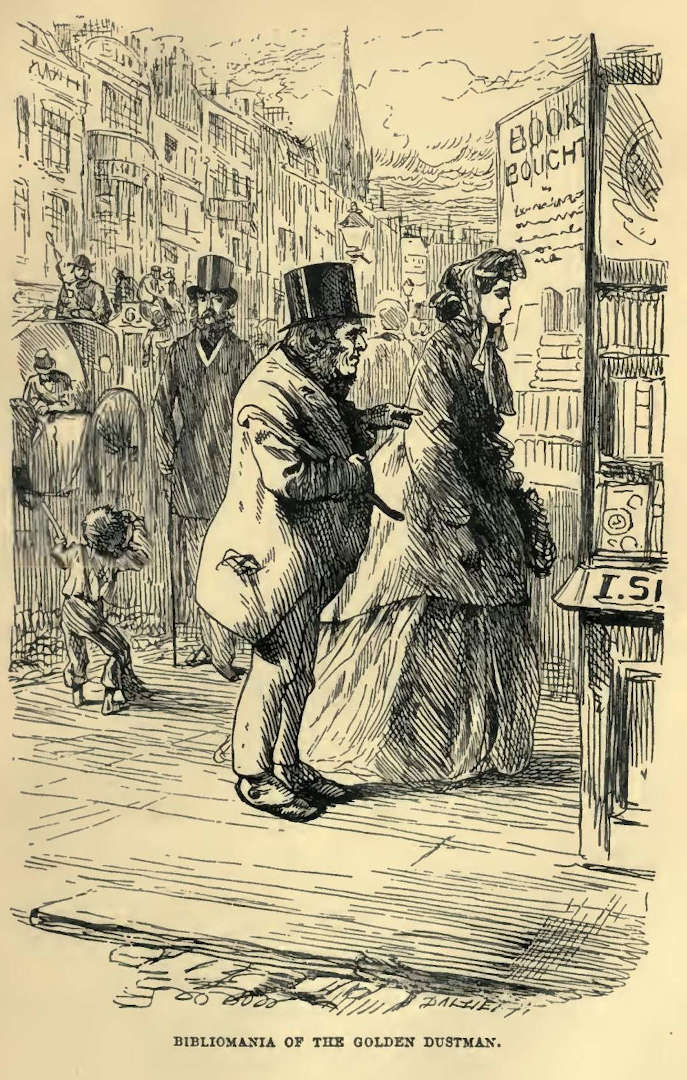
\includegraphics[scale=2.3]{03-05-01}

Behoves Mortimer Lightwood, therefore, to answer a dinner card from Mr
and Mrs Veneering requesting the honour, and to signify that Mr Mortimer
Lightwood will be happy to have the other honour. The Veneerings have
been, as usual, indefatigably dealing dinner cards to Society, and
whoever desires to take a hand had best be quick about it, for it is
written in the Books of the Insolvent Fates that Veneering shall make a
resounding smash next week. Yes. Having found out the clue to that great
mystery how people can contrive to live beyond their means, and having
over-jobbed his jobberies as legislator deputed to the Universe by the
pure electors of Pocket-Breaches, it shall come to pass next week that
Veneering will accept the Chiltern Hundreds, that the legal gentleman in
Britannia’s confidence will again accept the Pocket-Breaches Thousands,
and that the Veneerings will retire to Calais, there to live on Mrs
Veneering’s diamonds (in which Mr Veneering, as a good husband, has from
time to time invested considerable sums), and to relate to Neptune and
others, how that, before Veneering retired from Parliament, the House
of Commons was composed of himself and the six hundred and fifty-seven
dearest and oldest friends he had in the world. It shall likewise come
to pass, at as nearly as possible the same period, that Society will
discover that it always did despise Veneering, and distrust Veneering,
and that when it went to Veneering’s to dinner it always had
misgivings--though very secretly at the time, it would seem, and in a
perfectly private and confidential manner.

The next week’s books of the Insolvent Fates, however, being not yet
opened, there is the usual rush to the Veneerings, of the people who go
to their house to dine with one another and not with them. There is Lady
Tippins. There are Podsnap the Great, and Mrs Podsnap. There is Twemlow.
There are Buffer, Boots, and Brewer. There is the Contractor, who
is Providence to five hundred thousand men. There is the Chairman,
travelling three thousand miles per week. There is the brilliant genius
who turned the shares into that remarkably exact sum of three hundred
and seventy five thousand pounds, no shillings, and nopence.

To whom, add Mortimer Lightwood, coming in among them with a
reassumption of his old languid air, founded on Eugene, and belonging to
the days when he told the story of the man from Somewhere.

That fresh fairy, Tippins, all but screams at sight of her false
swain. She summons the deserter to her with her fan; but the deserter,
predetermined not to come, talks Britain with Podsnap. Podsnap always
talks Britain, and talks as if he were a sort of Private Watchman
employed, in the British interests, against the rest of the world. ‘We
know what Russia means, sir,’ says Podsnap; ‘we know what France wants;
we see what America is up to; but we know what England is. That’s enough
for us.’

However, when dinner is served, and Lightwood drops into his old place
over against Lady Tippins, she can be fended off no longer. ‘Long
banished Robinson Crusoe,’ says the charmer, exchanging salutations,
‘how did you leave the Island?’

‘Thank you,’ says Lightwood. ‘It made no complaint of being in pain
anywhere.’

‘Say, how did you leave the savages?’ asks Lady Tippins.

‘They were becoming civilized when I left Juan Fernandez,’ says
Lightwood. ‘At least they were eating one another, which looked like
it.’

‘Tormentor!’ returns the dear young creature. ‘You know what I mean, and
you trifle with my impatience. Tell me something, immediately, about the
married pair. You were at the wedding.’

‘Was I, by-the-by?’ Mortimer pretends, at great leisure, to consider.
‘So I was!’

‘How was the bride dressed? In rowing costume?’

Mortimer looks gloomy, and declines to answer.

‘I hope she steered herself, skiffed herself, paddled herself,
larboarded and starboarded herself, or whatever the technical term may
be, to the ceremony?’ proceeds the playful Tippins.

‘However she got to it, she graced it,’ says Mortimer.

Lady Tippins with a skittish little scream, attracts the general
attention. ‘Graced it! Take care of me if I faint, Veneering. He means
to tell us, that a horrid female waterman is graceful!’

‘Pardon me. I mean to tell you nothing, Lady Tippins,’ replies
Lightwood. And keeps his word by eating his dinner with a show of the
utmost indifference.

‘You shall not escape me in this way, you morose backwoodsman,’ retorts
Lady Tippins. ‘You shall not evade the question, to screen your friend
Eugene, who has made this exhibition of himself. The knowledge shall be
brought home to you that such a ridiculous affair is condemned by the
voice of Society. My dear Mrs Veneering, do let us resolve ourselves
into a Committee of the whole House on the subject.’

Mrs Veneering, always charmed by this rattling sylph, cries. ‘Oh yes!
Do let us resolve ourselves into a Committee of the whole House!
So delicious!’ Veneering says, ‘As many as are of that opinion, say
Aye,--contrary, No--the Ayes have it.’ But nobody takes the slightest
notice of his joke.

‘Now, I am Chairwoman of Committees!’ cries Lady Tippins.

[‘What spirits she has!’ exclaims Mrs Veneering; to whom likewise nobody
attends.)

‘And this,’ pursues the sprightly one, ‘is a Committee of the whole
House to what-you-may-call-it--elicit, I suppose--the voice of Society.
The question before the Committee is, whether a young man of very fair
family, good appearance, and some talent, makes a fool or a wise man of
himself in marrying a female waterman, turned factory girl.’

‘Hardly so, I think,’ the stubborn Mortimer strikes in. ‘I take the
question to be, whether such a man as you describe, Lady Tippins, does
right or wrong in marrying a brave woman (I say nothing of her beauty),
who has saved his life, with a wonderful energy and address; whom he
knows to be virtuous, and possessed of remarkable qualities; whom he has
long admired, and who is deeply attached to him.’

‘But, excuse me,’ says Podsnap, with his temper and his shirt-collar
about equally rumpled; ‘was this young woman ever a female waterman?’

‘Never. But she sometimes rowed in a boat with her father, I believe.’

General sensation against the young woman. Brewer shakes his head. Boots
shakes his head. Buffer shakes his head.

‘And now, Mr Lightwood, was she ever,’ pursues Podsnap, with his
indignation rising high into those hair-brushes of his, ‘a factory
girl?’

‘Never. But she had some employment in a paper mill, I believe.’

General sensation repeated. Brewer says, ‘Oh dear!’ Boots says, ‘Oh
dear!’ Buffer says, ‘Oh dear!’ All, in a rumbling tone of protest.

‘Then all I have to say is,’ returns Podsnap, putting the thing away
with his right arm, ‘that my gorge rises against such a marriage--that
it offends and disgusts me--that it makes me sick--and that I desire to
know no more about it.’

[‘Now I wonder,’ thinks Mortimer, amused, ‘whether YOU are the Voice of
Society!’)

‘Hear, hear, hear!’ cries Lady Tippins. ‘Your opinion of this
MESALLIANCE, honourable colleagues of the honourable member who has just
sat down?’

Mrs Podsnap is of opinion that in these matters there should be an
equality of station and fortune, and that a man accustomed to Society
should look out for a woman accustomed to Society and capable of bearing
her part in it with--an ease and elegance of carriage--that.’ Mrs
Podsnap stops there, delicately intimating that every such man should
look out for a fine woman as nearly resembling herself as he may hope to
discover.

[‘Now I wonder,’ thinks Mortimer, ‘whether you are the Voice!’)

Lady Tippins next canvasses the Contractor, of five hundred thousand
power. It appears to this potentate, that what the man in question
should have done, would have been, to buy the young woman a boat and a
small annuity, and set her up for herself. These things are a question
of beefsteaks and porter. You buy the young woman a boat. Very good. You
buy her, at the same time, a small annuity. You speak of that annuity in
pounds sterling, but it is in reality so many pounds of beefsteaks and
so many pints of porter. On the one hand, the young woman has the boat.
On the other hand, she consumes so many pounds of beefsteaks and so many
pints of porter. Those beefsteaks and that porter are the fuel to that
young woman’s engine. She derives therefrom a certain amount of power to
row the boat; that power will produce so much money; you add that to the
small annuity; and thus you get at the young woman’s income. That (it
seems to the Contractor) is the way of looking at it.

The fair enslaver having fallen into one of her gentle sleeps during the
last exposition, nobody likes to wake her. Fortunately, she comes
awake of herself, and puts the question to the Wandering Chairman. The
Wanderer can only speak of the case as if it were his own. If such a
young woman as the young woman described, had saved his own life, he
would have been very much obliged to her, wouldn’t have married her, and
would have got her a berth in an Electric Telegraph Office, where young
women answer very well.

What does the Genius of the three hundred and seventy-five thousand
pounds, no shillings, and nopence, think? He can’t say what he thinks,
without asking: Had the young woman any money?

‘No,’ says Lightwood, in an uncompromising voice; ‘no money.’

‘Madness and moonshine,’ is then the compressed verdict of the Genius.
‘A man may do anything lawful, for money. But for no money!--Bosh!’

What does Boots say?

Boots says he wouldn’t have done it under twenty thousand pound.

What does Brewer say?

Brewer says what Boots says.

What does Buffer say?

Buffer says he knows a man who married a bathing-woman, and bolted.

Lady Tippins fancies she has collected the suffrages of the whole
Committee (nobody dreaming of asking the Veneerings for their opinion),
when, looking round the table through her eyeglass, she perceives Mr
Twemlow with his hand to his forehead.

Good gracious! My Twemlow forgotten! My dearest! My own! What is his
vote?

Twemlow has the air of being ill at ease, as he takes his hand from his
forehead and replies.

‘I am disposed to think,’ says he, ‘that this is a question of the
feelings of a gentleman.’

‘A gentleman can have no feelings who contracts such a marriage,’
flushes Podsnap.

‘Pardon me, sir,’ says Twemlow, rather less mildly than usual, ‘I don’t
agree with you. If this gentleman’s feelings of gratitude, of respect,
of admiration, and affection, induced him (as I presume they did) to
marry this lady--’

‘This lady!’ echoes Podsnap.

‘Sir,’ returns Twemlow, with his wristbands bristling a little, ‘YOU
repeat the word; I repeat the word. This lady. What else would you call
her, if the gentleman were present?’

This being something in the nature of a poser for Podsnap, he merely
waves it away with a speechless wave.

‘I say,’ resumes Twemlow, ‘if such feelings on the part of this
gentleman, induced this gentleman to marry this lady, I think he is the
greater gentleman for the action, and makes her the greater lady. I beg
to say, that when I use the word, gentleman, I use it in the sense in
which the degree may be attained by any man. The feelings of a gentleman
I hold sacred, and I confess I am not comfortable when they are made the
subject of sport or general discussion.’

‘I should like to know,’ sneers Podsnap, ‘whether your noble relation
would be of your opinion.’

‘Mr Podsnap,’ retorts Twemlow, ‘permit me. He might be, or he might not
be. I cannot say. But, I could not allow even him to dictate to me on a
point of great delicacy, on which I feel very strongly.’

Somehow, a canopy of wet blanket seems to descend upon the company, and
Lady Tippins was never known to turn so very greedy or so very cross.
Mortimer Lightwood alone brightens. He has been asking himself, as to
every other member of the Committee in turn, ‘I wonder whether you are
the Voice!’ But he does not ask himself the question after Twemlow has
spoken, and he glances in Twemlow’s direction as if he were grateful.
When the company disperse--by which time Mr and Mrs Veneering have had
quite as much as they want of the honour, and the guests have had quite
as much as THEY want of the other honour--Mortimer sees Twemlow home,
shakes hands with him cordially at parting, and fares to the Temple,
gaily.



POSTSCRIPT

IN LIEU OF PREFACE


When I devised this story, I foresaw the likelihood that a class of
readers and commentators would suppose that I was at great pains to
conceal exactly what I was at great pains to suggest: namely, that Mr
John Harmon was not slain, and that Mr John Rokesmith was he. Pleasing
myself with the idea that the supposition might in part arise out
of some ingenuity in the story, and thinking it worth while, in the
interests of art, to hint to an audience that an artist (of whatever
denomination) may perhaps be trusted to know what he is about in his
vocation, if they will concede him a little patience, I was not alarmed
by the anticipation.

To keep for a long time unsuspected, yet always working itself out,
another purpose originating in that leading incident, and turning it to
a pleasant and useful account at last, was at once the most interesting
and the most difficult part of my design. Its difficulty was much
enhanced by the mode of publication; for, it would be very unreasonable
to expect that many readers, pursuing a story in portions from month
to month through nineteen months, will, until they have it before them
complete, perceive the relations of its finer threads to the whole
pattern which is always before the eyes of the story-weaver at his loom.
Yet, that I hold the advantages of the mode of publication to outweigh
its disadvantages, may be easily believed of one who revived it in the
Pickwick Papers after long disuse, and has pursued it ever since.

There is sometimes an odd disposition in this country to dispute as
improbable in fiction, what are the commonest experiences in fact.
Therefore, I note here, though it may not be at all necessary, that
there are hundreds of Will Cases (as they are called), far more
remarkable than that fancied in this book; and that the stores of the
Prerogative Office teem with instances of testators who have made,
changed, contradicted, hidden, forgotten, left cancelled, and left
uncancelled, each many more wills than were ever made by the elder Mr
Harmon of Harmony Jail.

In my social experiences since Mrs Betty Higden came upon the scene and
left it, I have found Circumlocutional champions disposed to be
warm with me on the subject of my view of the Poor Law. Mr friend Mr
Bounderby could never see any difference between leaving the Coketown
‘hands’ exactly as they were, and requiring them to be fed with turtle
soup and venison out of gold spoons. Idiotic propositions of a parallel
nature have been freely offered for my acceptance, and I have been
called upon to admit that I would give Poor Law relief to anybody,
anywhere, anyhow. Putting this nonsense aside, I have observed a
suspicious tendency in the champions to divide into two parties; the
one, contending that there are no deserving Poor who prefer death by
slow starvation and bitter weather, to the mercies of some Relieving
Officers and some Union Houses; the other, admitting that there are such
Poor, but denying that they have any cause or reason for what they do.
The records in our newspapers, the late exposure by THE LANCET, and the
common sense and senses of common people, furnish too abundant evidence
against both defences. But, that my view of the Poor Law may not be
mistaken or misrepresented, I will state it. I believe there has been
in England, since the days of the STUARTS, no law so often infamously
administered, no law so often openly violated, no law habitually so
ill-supervised. In the majority of the shameful cases of disease and
death from destitution, that shock the Public and disgrace the country,
the illegality is quite equal to the inhumanity--and known language
could say no more of their lawlessness.

On Friday the Ninth of June in the present year, Mr and Mrs Boffin (in
their manuscript dress of receiving Mr and Mrs Lammle at breakfast)
were on the South Eastern Railway with me, in a terribly destructive
accident. When I had done what I could to help others, I climbed back
into my carriage--nearly turned over a viaduct, and caught aslant upon
the turn--to extricate the worthy couple. They were much soiled, but
otherwise unhurt. The same happy result attended Miss Bella Wilfer on
her wedding day, and Mr Riderhood inspecting Bradley Headstone’s red
neckerchief as he lay asleep. I remember with devout thankfulness that I
can never be much nearer parting company with my readers for ever, than
I was then, until there shall be written against my life, the two words
with which I have this day closed this book.

-- THE END.

September 2nd, 1865.
